% @author: Achmad Zainur Rozzykin
% 

%------------------------------------------------------------------------------------%
% Tipe dokumen, menggunakan book-edited --> template, dengan satu kolom, cetak satu sisi, A4 dll. 
%
\documentclass[oneside, onecolumn, fleqn, a4paper, 12pt]{template_layout}

%------------------------------------------------------------------------------------%
% Package yang digunakan
% Digunakan untuk memasukan gambar ke laporan.
\usepackage{graphicx}
\usepackage{subfigure}
\usepackage{booktabs,caption,fixltx2e}
\usepackage[flushleft]{threeparttable}

% The geometry package controls the overall margins and text area of the 
% document. The package must be called in the preamble of the document and specified when called.
\usepackage[left=4cm, right=3cm, top=3cm, bottom=3cm]{geometry}

% Membantu penulisan notasi matematika terutama untuk dokumen dengan banyak rumus.
\usepackage{amsmath}

% The package hyperref provides LaTeX the ability to create hyperlinks within the document
\usepackage{hyperref}

% The url package allows spacing and line breaks that result in intelligent 
% printing of email addresses, hypertext links, and path or directory addresses. 
\usepackage{url}

% agar gambar tidak selalu di atas atau di bawah
\usepackage{float}
\floatplacement{figure}{H}
\floatplacement{table}{H}

% merger baris di tabel
\usepackage{multirow}
\usepackage{longtable}
\usepackage{color, openbib, rotate, amsfonts, amsmath, amssymb, amstext}
\usepackage{makeidx}
\usepackage[mathcal]{euscript}
\usepackage[bahasai]{babel}
\usepackage{listings}

%------------------------------------------------------------------------------------%
% hyphenation
%
% Hyphenation untuk Indonesia 
% @author  Ridlo Wahyudi Wibowo
% 
% Tambahkan cara pemenggalan kata-kata yang salah dipenggal secara otomatis 
% oleh LaTeX. Jika kata tersebut dapat dipenggal dengan benar, maka tidak 
% perlu ditambahkan dalam berkas ini. Tanda pemenggalan kata menggunakan 
% tanda '-'; contoh:
% menarik
%   --> pemenggalan: me-na-rik
%

\hyphenation{
    % alphabhet A
    a-na-li-sa a-tur 
    a-pli-ka-si
    a-kan 
    % alphabhet B
    bumi
    ba-ngun-an 
    be-be-ra-pa 
    be-ru-pa
    ber-ge-rak
    ber-ke-lan-jut-an 
    ber-pe-nga-ruh 
    ber-dasar-kan
    bong-kah-an
    % alphabhet C
    ca-ri
    % alphabhet D
    di-sim-pan di-pim-pin de-ngan da-e-rah di-ba-ngun da-pat di-nya-ta-kan 
    di-sim-bol-kan di-pi-lih di-li-hat de-fi-ni-si
    di-ban-ding-kan
    di-si-mu-la-si-kan
    di-li-bat-kan
    di-se-bab-kan
    di-la-ku-kan
    di-je-las-kan
    di-tambah-kan
    di-temu-kan
    di-masuk-kan
    di-distribusi-kan
    di-harap-kan
    di-tunjuk-kan
    di-kata-kan
    di-be-da-kan
    Desktop
    di-pre-dik-si
    % alphabhet E
    e-ner-gi eks-klu-sif
    error
    % alphabhet F
    fa-si-li-tas
    fitting
    % alphabhet G
    ga-bung-an ge-rak
    ge-ta-ran
    % alphabhet H
    ha-lang-an
    Head
    % alphabhet I
    % alphabhet J
    % alphabhet K
    ke-hi-lang-an
		ke-sta-bil-an
    ku-ning 
    kua-li-tas ka-me-ra ke-mung-kin-an ke-se-pa-ham-an
    kur-va
    % alphabhet L
    LINEAR
    ling-kung-an
    lu-mi-no-si-tas
    % alphabhet M
    me-neng-ah
    me-dan
    meng-a-tas-i me-mung-kin-kan me-nge-na-i me-ngi-rim-kan 
    meng-u-bah meng-a-dap-ta-si me-nya-ta-kan mo-di-fi-ka-si
    meng-a-tur
    meng-gu-na-kan
		meng-ha-sil-kan
		me-nam-bah-kan
		me-nen-tu-kan
    me-nun-juk-kan
    mem-per-li-hat-kan		
    men-je-las-kan
    me-nye-bab-kan
    me-ru-pa-kan
    me-li-bat-kan
    meng-a-ki-bat-kan
    mengajari
    mengelilingi
    men-cipta-kan
    me-model-kan
    me-manfaat-kan
    mem-be-ri-kan
    ma-sing-ma-sing
    me-nger-ja-kan
    % alphabhet N
    nya-ta non-eks-klu-sif
    % alphabhet O
    neo-wise
    % alphabhet P
    pro-grade
	pe-nye-rap-an 
	pe-ngon-trol
    pe-mo-del-an
    pe-ran  pe-ran-an-nya
    pem-rog-ram-an
    pem-ba-ngun-an pre-si-den pe-me-rin-tah prio-ri-tas peng-am-bil-an 
    peng-ga-bung-an pe-nga-was-an pe-ngem-bang-an 
    pe-nga-ruh pa-ra-lel-is-me per-hi-tung-an per-ma-sa-lah-an 
    pen-ca-ri-an peng-struk-tur-an
    per-ban-ding-an
    per-kuliah-an
    pe-mro-gram-an
    pe-ri-o-de
    para-me-ter
    % alphabhet Q
    % alphabhet R
    ran-cang-an
    re-tro-grade
    % alphabhet S
    si-mu-la-si sa-ngat sur-vey sur-vei
    se-dang-kan
    stag-nan
		sub-sti-tu-si
    % alphabhet T
    te-ngah
    ter-da-pat
    tisserand
    trans-ver-sal
		tri-angu-lar
    % alphabhet U
    % alphabhet V
    % alphabhet W
    WIMPs
    % alphabhet X
    % alphabhet Y
    % alphabhet Z
    % special
}

%------------------------------------------------------------------------------------%
% Mendefinisikan perintah tambahan
%
\AtBeginDocument{\renewcommand{\bibname}{DAFTAR PUSTAKA}}
\AtBeginDocument{\renewcommand{\contentsname}{DAFTAR ISI}}
\AtBeginDocument{\renewcommand{\listfigurename}{DAFTAR GAMBAR}}
\AtBeginDocument{\renewcommand{\listtablename}{DAFTAR TABEL}}
\renewcommand{\thefootnote}{\arabic{footnote}}
\renewcommand{\index}{\arabic{indeks}}
\newcommand{\pic}{Gambar}
\newcommand{\tab}{Tabel}
\newcommand{\equ}{Persamaan}

%menghilangkan numbering di daftar pustaka
\makeatletter
\renewcommand\@biblabel[1]{}
\makeatother

%------------------------------------------------------------------------------------%
% Mulai menulis dokumen
%
\begin{document}
\frontmatter
\begin{titlepage}
\begin{center}

\textbf{\large{JUDUL TUGAS AKHIR
}}\\

\vspace{3cm}

\textbf{\large{TUGAS AKHIR}}\\

\textbf{Karya tulis sebagai salah satu syarat \\
untuk memperoleh gelar Sarjana dari \\
Institut Teknologi Bandung}\\

\vspace{2cm}
\textbf{Oleh}

\textbf{\large{Author\\
103xxxxx}}\\

\vspace{2.0cm}
%\textbf{\large{KELOMPOK KEILMUAN ASTRONOMI}}
%\vspace{1.5cm}

\begin{figure}[!h]
\centering
%\hspace{5cm}

\includegraphics[width=2.5cm, height=3.5cm]{pics/gajah.jpg}
\end{figure}

\vspace{2.0cm}

\textbf{\normalsize{PROGRAM STUDI SARJANA ASTRONOMI}\\
\small{FAKULTAS MATEMATIKA DAN ILMU PENGETAHUAN ALAM}\\
\large{INSTITUT TEKNOLOGI BANDUNG \\
2018}}

\end{center}
\end{titlepage}
\newpage
\pagestyle{empty}
\begin{center}
\textbf{\large{JUDUL TUGAS AKHIR}}\\

\vspace{2cm}

Oleh\\
\large{\textbf{Author\\
NIM 103xxxxx}\\

\vspace{1cm}

Program Studi Astronomi\\
Institut Teknologi Bandung}

\vspace{2cm}

Menyetujui,\\
Bandung, DD MMMM YYYY\\
Dosen Pembimbing\\

\vspace{2.5cm}

NAMA DOSBING \\
NIP DOSBING
\end{center}

\vspace{1cm}

\begin{flushleft}
Tim Penguji:\\
1. Penguji 1\\
2. Penguji 2\\
3. Penguji 3\\
\end{flushleft}



\newpage
% mulai penomeran romawi
\pagenumbering{roman}
\chapter{PEDOMAN PENGGUNAAN \mbox{TUGAS AKHIR}}
\label{sec:PEDOMAN PENGGUNAAN TUGAS AKHIR}
\vspace{1.0cm}

Tugas Akhir Sarjana yang tidak dipublikasikan terdaftar dan tersedia di Perpustakaan Institut Teknologi Bandung, dan terbuka untuk umum dengan ketentuan bahwa hak cipta ada pada penulis dengan mengikuti aturan HaKI yang  berlaku di Institut Teknologi Bandung. Referensi kepustakaan diperkenankan dicatat, tetapi pengutipan atau peringkasan hanya dapat dilakukan seizin penulis dan harus disertai dengan kebiasaan ilmiah untuk menyebutkan sumbernya.

Memperbanyak atau menerbitkan sebagian atau seluruh Tugas Akhir harus atas izin Program Studi Sarjana Astronomi, Institut Teknologi Bandung.

\chapter{ABSTRAK}
\vspace{0.05cm}

Lorem ipsum dolor sit amet, eos at erat iracundia. Cu sea errem nobis persecuti. Te diam causae sanctus est, vocent dolorum abhorreant ex nam. An mei vidit consul mediocrem, nam quaeque habemus an, vidit causae explicari sea ei.Lorem minimum referrentur in vis, enim mundi vix ea, ei nam tation eloquentiam. Ignota animal menandri et quo, ei reque veritus qui. At novum omittantur eos. Vim denique periculis iracundia te, rationibus philosophia id duo. Ius justo insolens pertinax eu. \par

Sed et mundi dissentias. Nam quidam delenit deleniti ad, cum ea iudico volumus epicuri. Mea viris equidem an. Et vix soleat aperiri tractatos.Eos quas graeco ancillae ea, eu torquatos tincidunt constituam pro. Ei his odio liber intellegam. Ex everti lobortis usu, has ex esse fabellas invidunt. Vix et veniam omnesque, vim ea aeterno invenire erroribus, per choro hendrerit deseruisse an. \par 

Ei mea dico assentior, usu at tation bonorum definitionem, nam quas malorum habemus an. Te justo propriae quo, altera admodum tincidunt quo no. Cibo officiis constituam ei pro, in delectus deserunt qui, et quod accumsan quo. Apeirian gloriatur delicatissimi nec ex, usu delenit offendit principes ei. Putent aperiri gubergren ex vim, wisi ludus vis cu. Nostrud hendrerit cu vis. Eos eu iuvaret graecis. Est ea accusata quaestio, reque nulla dicunt eum ne. Ne cum quod oportere, labore laoreet platonem mea cu, no mei dicat lucilius democritum. Eu timeam evertitur constituam mea, id ancillae placerat pro. Has ad choro percipitur. Cu ullum causae voluptua sed.\par
\vspace{0.05cm}
\textbf{Kata kunci}: Lorem, ipsum, dolor, sit amet
\chapter{ABSTRACT}
\vspace{0.05cm}

Lorem ipsum dolor sit amet, eos at erat iracundia. Cu sea errem nobis persecuti. Te diam causae sanctus est, vocent dolorum abhorreant ex nam. An mei vidit consul mediocrem, nam quaeque habemus an, vidit causae explicari sea ei.Lorem minimum referrentur in vis, enim mundi vix ea, ei nam tation eloquentiam. Ignota animal menandri et quo, ei reque veritus qui. At novum omittantur eos. Vim denique periculis iracundia te, rationibus philosophia id duo. Ius justo insolens pertinax eu. \par

Sed et mundi dissentias. Nam quidam delenit deleniti ad, cum ea iudico volumus epicuri. Mea viris equidem an. Et vix soleat aperiri tractatos.Eos quas graeco ancillae ea, eu torquatos tincidunt constituam pro. Ei his odio liber intellegam. Ex everti lobortis usu, has ex esse fabellas invidunt. Vix et veniam omnesque, vim ea aeterno invenire erroribus, per choro hendrerit deseruisse an. \par 

Ei mea dico assentior, usu at tation bonorum definitionem, nam quas malorum habemus an. Te justo propriae quo, altera admodum tincidunt quo no. Cibo officiis constituam ei pro, in delectus deserunt qui, et quod accumsan quo. Apeirian gloriatur delicatissimi nec ex, usu delenit offendit principes ei. Putent aperiri gubergren ex vim, wisi ludus vis cu. Nostrud hendrerit cu vis. Eos eu iuvaret graecis. Est ea accusata quaestio, reque nulla dicunt eum ne. Ne cum quod oportere, labore laoreet platonem mea cu, no mei dicat lucilius democritum. Eu timeam evertitur constituam mea, id ancillae placerat pro. Has ad choro percipitur. Cu ullum causae voluptua sed.\par
\vspace{0.05cm}
\textbf{Kata kunci}: Lorem, ipsum, dolor, sit amet
\chapter*{}


\vspace{5cm}

\begin{quote}
\begin{center}
\textit{Di balik kesuksesan seseorang, \\
bukan hanya terdapat orang tua dan guru yang hebat, \\
tetapi terdapat pula teman-teman yang berjiwa malaikat. }
\end{center}
\end{quote}




\chapter*{}


\vspace*{\fill}

\begin{quote}
\begin{flushright}
\begin{small}
\textit{Iman tanpa ilmu bagaikan lentera di tangan bayi. Namun ilmu tanpa iman,bagaikan lentera di tangan pencuri. (Buya Hamka)\\}

\vspace{2cm}
\textit{Ilmu seperti udara. Ia begitu banyak di sekeliling kita. Kamu bisa mendapatkannya dimanapun dan kapanpun. (Socrates)\\}
\end{small}
\end{flushright}
\end{quote}



\pagestyle{plain}
\chapter{KATA PENGANTAR}
\vspace{1.0cm}

\textit{Assalamu’alaikum Wr. Wb.} \\

	Puji syukur Penulis panjatkan kepada Tuhan Yang Maha Esa, Allah SWT atas rahmat dan anugerah-Nya sehingga Penulis dapat menyelesaikan Tugas Akhir yang berjudul “JUDUL TUGAS AKHIR”. Tanpa petunjuk dan pertolongan-Nya, Penulis tidak dapat sampai pada titik ini.  \\
	
	Penulis menyadari bahwa selama pengerjaan Tugas Akhir banyak mendapatkan motivasi dan dukungan dari berbagai pihak. Oleh karena itu, Penulis mengucapkan terima kasih kepada orang tua Penulis yang telah banyak memberikan dukungan moral dan material sehingga Penulis dapat menyelesaikan Tugas Akhir. Selain itu, Penulis juga mengucapkan terima kasih kepada:

\begin{enumerate}
	\item NAMA DOSBING selaku dosen pembimbing atas kesabaran beliau dalam membimbing Penulis untuk memahami materi Tugas Akhir. Selain itu, saya mengucapkan terima kasih atas motivasi, nasehat, dan ilmu baik akademik maupun non-akademik yang telah Bapak/Ibu NAMA DOSBING berikan selama ini. 
	\item PENGUJI 1, PENGUJI 2 dan PENGUJI 3 selaku dosen penguji atas saran dan kritikan yang membangun sehingga Tugas Akhir Penulis dapat menjadi lebih baik. 
	\item DOSEN WALI selaku dosen wali Penulis yang telah membimbing Penulis dan banyak memberikan nasehat selama tiga tahun ini. 
	\item Dosen Program Studi Sarjana Astronomi yang telah memberikan berbagai ilmu yang bermanfaat selama Penulis menjadi mahasiswa Astronomi. 
	\item Staf Tata Usaha (Ibu Isna, Ibu Ati, dan Pak Yayan) yang telah banyak membantu Penulis dalam mengurus administrasi akademik dan Ibu Ina yang telah membantu Penulis dalam mendapatkan buku-buku yang menunjang selama Penulis kuliah maupun selama mengerjakan Tugas Akhir.  
	\item Keluarga besar Penulis ...
	\item ....
	\item Pihak-pihak lain yang telah membantu Penulis dan tidak dapat Penulis sebutkan satu-persatu. 
\end{enumerate}
Penulis menyadari bahwa Tugas Akhir ini masih terdapat banyak kekurangan. Oleh karena itu, Penulis sangat mengharapkan kritik dan saran agar Tugas Akhir ini menjadi lebih baik. Penulis juga berharap semoga Tugas Akhir ini dapat bermanfaat bagi siapapun yang membutuhkan referensi baik dalam mengerjakan Tugas Akhir maupun penelitian yang serupa terutama dalam bidang SESUAI DENGAN KELOMPOK KEAHLIAN.\\
\vspace{1cm}
\begin{flushright}
Bandung, DD MMMM YYYY\\
\vspace{2cm}
Wulandari
\end{flushright}

\chapter*{SANWACANA}
\vspace{1.0cm}

Penulis mengucapkan terima kasih kepada ....  

\tableofcontents
\listoftables
\listoffigures
\mainmatter
% mulai penomeran romawi
\pagenumbering{arabic}
\chapter{PENDAHULUAN}
\vspace{1.0cm}

%-----------------------------------------------------------------------------%
\section{Latar Belakang}
%-----------------------------------------------------------------------------%

Lorem ipsum dolor sit amet, odio utroque definiebas ut quo, delenit omittam ne nec. Ius in assentior consectetuer, eos id malorum prodesset accommodare. Quot explicari definitionem eam eu, magna adipiscing eu nec. Dicta dicam sanctus vis cu, vel ne autem civibus facilisis. Ad dicat dolores pro, sea ex wisi justo possim, alienum reprehendunt vim ad. Sed quas verear ea, et wisi timeam percipitur his. Probo scaevola vim cu.\\

Ea vix assum recusabo, fabulas maiestatis ei sed. Pri wisi omnesque ex. Eum ea mundi laoreet appellantur, postea vidisse efficiantur sed ad. Duo case civibus ea, no pro recusabo scripserit. Has id audire deterruisset. Eam cu cibo exerci, et facilisis consetetur vix, mel an soleat ceteros.\\

Ex prima eirmod vulputate pri, eum no essent mandamus. Albucius accusamus salutatus vix at, assum ullamcorper ex sea. Vis eleifend consetetur ut, ex ius verear rationibus sadipscing. Meliore assentior sit cu. Vidisse omittantur vim ne. Regione accusam vituperatoribus vel ut, et sit commodo concludaturque.\\

%-----------------------------------------------------------------------------%	 
\section{Rumusan Masalah}
%-----------------------------------------------------------------------------%
Berdasarkan latar belakang yang telah diuraikan, dirumuskan masalah yang akan dibahas dalam Tugas Akhir ini sebagai berikut:
\begin{enumerate}
	\item Rumusan masalah pertama?
\pagebreak	
	\item Rumusan masalah kedua?
\end{enumerate}

%-----------------------------------------------------------------------------%
\section{Tujuan}
%-----------------------------------------------------------------------------%

Tujuan dari Tugas Akhir ini adalah untuk ...

%-----------------------------------------------------------------------------%
\section{Metode Penelitian dan Teknik Pengumpulan Data}
%-----------------------------------------------------------------------------%

Metode penelitian dalam Tugas Akhir ini adalah ..., yaitu:
\begin{enumerate}
	\item metode 1.
	\item metode 2. 
	\item metode 3.
\end{enumerate}
	
	Adapun teknik pengumpulan data yang digunakan dalam Tugas Akhir ini adalah ... \\

%-----------------------------------------------------------------------------%
\section{Sistematika Penulisan}
%-----------------------------------------------------------------------------%

	Tugas Akhir ini terdiri dari lima bab. Bab I merupakan bab pendahuluan yang terdiri atas latar belakang pemilihan topik Tugas Akhir, rumusan masalah, tujuan dari Tugas Akhir, metode penelitian dan teknik pengumpulan data yang digunakan dalam Tugas Akhir, serta sistematika dalam penulisan Tugas Akhir. Bab II membahas tentang teori dasar. Bab III membahas mengenai data yang digunakan dalam Tugas Akhir beserta metode pengolahannya. Bab IV membahas mengenai hasil dari pengolahan data beserta analisisnya. Bab V terdiri atas simpulan dan saran Penulis terhadap permasalahan yang dibahas dalam Tugas Akhir ini. \\

\chapter{TEORI DASAR}
\vspace{1.0cm}

%-----------------------------------------------------------------------------%
\section{Teori ke-1}
%-----------------------------------------------------------------------------%
Lorem ipsum dolor sit amet, odio utroque definiebas ut quo, delenit omittam ne nec. Ius in assentior consectetuer, eos id malorum prodesset accommodare. Quot explicari definitionem eam eu, magna adipiscing eu nec. Dicta dicam sanctus vis cu, vel ne autem civibus facilisis. Ad dicat dolores pro, sea ex wisi justo possim, alienum reprehendunt vim ad. Sed quas verear ea, et wisi timeam percipitur his. Probo scaevola vim cu. Ea vix assum recusabo, fabulas maiestatis ei sed. Pri wisi omnesque ex. Eum ea mundi laoreet appellantur, postea vidisse efficiantur sed ad. Duo case civibus ea, no pro recusabo scripserit. Has id audire deterruisset. Eam cu cibo exerci, et facilisis consetetur vix, mel an soleat ceteros. Ex prima eirmod vulputate pri, eum no essent mandamus. Albucius accusamus salutatus vix at, assum ullamcorper ex sea. Vis eleifend consetetur ut, ex ius verear rationibus sadipscing. Meliore assentior sit cu. Vidisse omittantur vim ne. Regione accusam vituperatoribus vel ut, et sit commodo concludaturque. (lihat Gambar \ref{fig:garputala}). \\
\begin{figure}[H] 
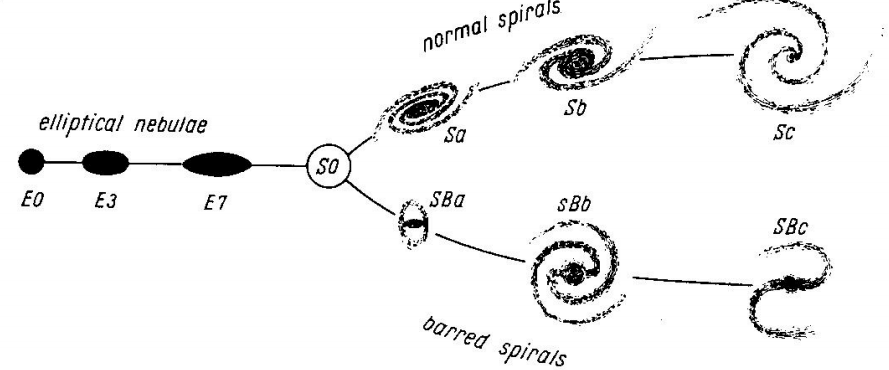
\includegraphics[scale=0.45]{pics/garputala.png}
\caption[Diagram garpu tala Hubble]{Diagram garpu tala Hubble yang menunjukkan klasifikasi galaksi elips, spiral, dan lentikular (Sumber: Hubble, 1958)}
\label{fig:garputala}
\centering
\end{figure}
	Lorem ipsum dolor sit amet, odio utroque definiebas ut quo, delenit omittam ne nec. Ius in assentior consectetuer, eos id malorum prodesset accommodare. Quot explicari definitionem eam eu, magna adipiscing eu nec. Dicta dicam sanctus vis cu, vel ne autem civibus facilisis. Ad dicat dolores pro, sea ex wisi justo possim, alienum reprehendunt vim ad. Sed quas verear ea, et wisi timeam percipitur his. Probo scaevola vim cu.\\
	
	Ea vix assum recusabo, fabulas maiestatis ei sed. Pri wisi omnesque ex. Eum ea mundi laoreet appellantur, postea vidisse efficiantur sed ad. Duo case civibus ea, no pro recusabo scripserit. Has id audire deterruisset. Eam cu cibo exerci, et facilisis consetetur vix, mel an soleat ceteros.\\
	
	Ex prima eirmod vulputate pri, eum no essent mandamus. Albucius accusamus salutatus vix at, assum ullamcorper ex sea. Vis eleifend consetetur ut, ex ius verear rationibus sadipscing. Meliore assentior sit cu. Vidisse omittantur vim ne. Regione accusam vituperatoribus vel ut, et sit commodo concludaturque.\\
	
\begin{figure}[H] 
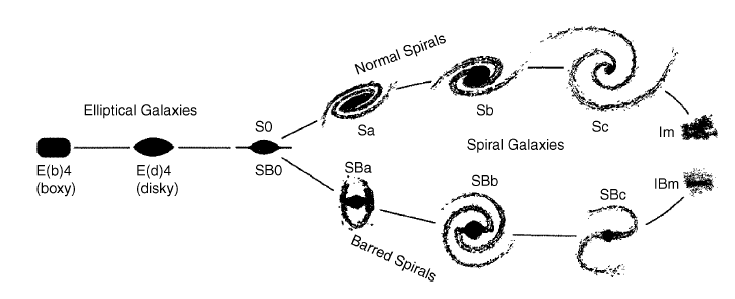
\includegraphics[scale=0.55]{pics/garputala2.png}
\caption[Diagram garpu tala Hubble hasil modifikasi]{Diagram garpu tala Hubble yang dimodifikasi, yang mengklasifikasikan galaksi menjadi galaksi elips, lentikular, spiral dan iregular (Sumber: Schneider,  2010)}
\label{fig:garputala2}
\centering
\end{figure}
%-----------------------------------------------------------------------------%
\section{Fotometri Galaksi Spiral}
%-----------------------------------------------------------------------------%
\subsection{Fotometri Galaksi}
%-----------------------------------------------------------------------------%
Lorem ipsum dolor sit amet, odio utroque definiebas ut quo, delenit omittam ne nec. Ius in assentior consectetuer, eos id malorum prodesset accommodare. Quot explicari definitionem eam eu, magna adipiscing eu nec. Dicta dicam sanctus vis cu, vel ne autem civibus facilisis. Ad dicat dolores pro, sea ex wisi justo possim, alienum reprehendunt vim ad. Sed quas verear ea, et wisi timeam percipitur his. Probo scaevola vim cu. \\

	Ea vix assum recusabo, fabulas maiestatis ei sed. Pri wisi omnesque ex. Eum ea mundi laoreet appellantur, postea vidisse efficiantur sed ad. Duo case civibus ea, no pro recusabo scripserit. Has id audire deterruisset. Eam cu cibo exerci, et facilisis consetetur vix, mel an soleat ceteros.

\begin{equation} \label{kecerlangan}
I=\dfrac{F}{\alpha^{2}}=\dfrac{\dfrac{L}{4 \pi d^{2}}}{\bigg(\dfrac{D}{d} \bigg)^{2}}=\dfrac{L}{4 \pi D^{2}}
\end{equation}
dengan  $F$ merupakan kecerlangan semu. $L$ merupakan luminositas galaksi dan $D$ merupakan luas galaksi yang diamati pada jarak $d$ dan sudut ruang $\alpha$. Untuk galaksi yang memiliki piringan datar, kecerlangan permukaan berbanding terbalik dengan $\cos i$, $I \propto \dfrac{1}{\cos i}$. \\

	
\chapter{PENGOLAHAN DATA}
\vspace{1.0cm}

%-----------------------------------------------------------------------------%
\section{METODE 1}
%-----------------------------------------------------------------------------%
	Medan magnet terdeteksi hampir pada setiap objek astrofisika, mulai dari planet hingga pulsar, maupun pada struktur dengan skala yang lebih besar seperti  galaksi. Observasi medan magnet galaksi menunjukkan bahwa keberadaan medan magnet memerankan bagian penting dalam evolusi galaksi dan pembentukan struktur skala besar. Selain itu, medan magnet berperan penting dalam dinamika gas pada awan molekul. Dengan medan magnet yang kuat, beberapa inti awan terbentuk dengan massa yang besar. Medan magnet juga mengontrol densitas dan perambatan berkas kosmik (\textit{cosmic rays}). Bersama dengan berkas kosmik, medan magnet dapat menghasilkan tekanan untuk mempercepat aliran gas panas, khususnya dalam galaksi dengan laju pembentukan bintang yang tinggi pada awal alam semesta. \\
	

\begin{table}[H] 
\begin{center}
\caption[Hasil \textit{Fitting} Kurva Rotasi M31 dengan dan tanpa Medan Magnet]{Hasil \textit{Fitting} Kurva Rotasi tanpa \textit{Dark Matter} (hanya Medan Magnet), dengan \textit{Dark Matter}, dan dengan Kontribusi Medan Magnet dan \textit{Dark Matter} untuk $r\geq 3$ kpc (sumber: Ruiz-Granados et al., 2012)}
\begin{tabular}{ccc}
\hline
Model (Parameter) & $\chi^{2}$ untuk \textit{Best-fit} & \textit{Reduced-}$\chi^{2}$ \\
\hline
MAG ($r_{1}$) & 4.37 & 0.34 \\
ISO tanpa MAG ($\rho_{0}, R_{h}$) & 8.81 & 0.68 \\
ISO dengan MAG ($r_{1}$, $\rho_{0}, R_{h}$) & 4.39 & 0.34 \\
\hline
\end{tabular}
\label{table:fitting}
\end{center}
\end{table} 
\chapter{HASIL DAN ANALISIS}
\vspace{1.0cm}

%-----------------------------------------------------------------------------%
\section{ANALISIS 1}
%-----------------------------------------------------------------------------%
Lorem ipsum dolor sit amet, odio utroque definiebas ut quo, delenit omittam ne nec. Ius in assentior consectetuer, eos id malorum prodesset accommodare. Quot explicari definitionem eam eu, magna adipiscing eu nec. Dicta dicam sanctus vis cu, vel ne autem civibus facilisis. Ad dicat dolores pro, sea ex wisi justo possim, alienum reprehendunt vim ad. Sed quas verear ea, et wisi timeam percipitur his. Probo scaevola vim cu. \\

Ea vix assum recusabo, fabulas maiestatis ei sed. Pri wisi omnesque ex. Eum ea mundi laoreet appellantur, postea vidisse efficiantur sed ad. Duo case civibus ea, no pro recusabo scripserit. Has id audire deterruisset. Eam cu cibo exerci, et facilisis consetetur vix, mel an soleat ceteros.\\

Ex prima eirmod vulputate pri, eum no essent mandamus. Albucius accusamus salutatus vix at, assum ullamcorper ex sea. Vis eleifend consetetur ut, ex ius verear rationibus sadipscing. Meliore assentior sit cu. Vidisse omittantur vim ne. Regione accusam vituperatoribus vel ut, et sit commodo concludaturque.\\
\begin{itemize}
\item $(\frac{M}{L})_{disk}$ = 0,939 $\pm$ 0,006 $\frac{M_{\odot}}{L_{\odot}}$
\item $(\frac{M}{L})_{bulge}$ = 1,057 $\pm$ 0,00832 $\frac{M_{\odot}}{L_{\odot}}$
\item $R_{c}$ = 5,260 $\pm$ 0,011 kpc
\item $\rho_{h}(R_{c})$ = 0,045 $\pm$ 0,00003 $\frac{M_{\odot}}{pc^{3}}$
\item $\chi_{\nu}^{2}$ = 1,383 
\end{itemize}
\begin{figure}[H]
\centering 
\includegraphics[scale=0.6]{pics/dekom2841.png}
\caption[Plot Kurva Rotasi Galaksi NGC 2841 tanpa Medan Magnet]{Dekomposisi kurva rotasi NGC 2841 dengan tiga komponen galaksi, yaitu piringan bintang, gas, \textit{bulge} dan \textit{halo dark matter}.}
\label{fig:ngc2841}
\end{figure}

%-----------------------------------------------------------------------------%
\section{ANALISIS}
%-----------------------------------------------------------------------------%
\textit{Fitting} kurva rotasi NGC 7331 untuk kasus pertama, kedua dan ketiga dilakukan dengan metode yang sama seperti \textit{fitting} kurva rotasi NGC 2841 maupun NGC 6964. Gambar \ref{fig:ngc7331} menunjukkan hasil \textit{fitting} kurva rotasi untuk kasus pertama. \\
\begin{figure}[H]
\centering 
\includegraphics[scale=0.6]{pics/dekom7331.png}
\caption[Plot Kurva Rotasi NGC 7331 tanpa Medan Magnet]{Dekomposisi kurva rotasi NGC 7331 dengan menggunakan komponen piringan, gas, \textit{bulge}, dan \textit{halo dark matter}.}
\label{fig:ngc7331}
\end{figure}
Parameter-parameter yang dihasilkan dari \textit{fitting} kurva rotasi tersebut adalah sebagai berikut:
\begin{itemize}
\item $(\frac{M}{L})_{disk}$ = 0,698 $\pm$ 0,001 $\frac{M_{\odot}}{L_{\odot}}$
\item $(\frac{M}{L})_{bulge}$ = 0,702 $\pm$ 0,002 $\frac{M_{\odot}}{L_{\odot}}$
\item $R_{c}$ = 19,820 $\pm$ 0,099 kpc
\item $\rho_{h}(R_{c})$ = 0,005 $\pm$ 0,00001 $\frac{M_{\odot}}{pc^{3}}$
\item $\chi_{\nu}^{2}$ = 3,357
\end{itemize}
	Seperti halnya dengan NGC 2841 dan NGC 6946, \textit{fitting} kurva rotasi pada kasus kedua diawali dengan melakukan \textit{fitting} profil medan magnet dalam arah azimuthal yang menghasilkan parameter $B_{1}$ dan $r_{1}$. Gambar \ref{fig:fitngc7331} menunjukkan hasil fitting profil medan magnet dalam arah azimuthal.\\
\begin{figure}[H]
\centering 
\includegraphics[scale=0.6]{pics/fitting7331.png}
\caption[Plot \textit{fitting} Profil Medan Magnet Azimuthal Galaksi NGC 7331]{Hasil \textit{fitting} profil medan magnet dalam arah azimuthal untuk NGC 7331.}
\label{fig:fitngc7331}
\end{figure}
	Berdasarkan \textit{fitting} profil medan magnet, didapatkan nilai $B_{1}$ sebesar 1002,05 $\pm$ 0,24 $\mu$G dan nilai  sebesar 0,14 $\pm$ 0,0005 kpc dengan \textit{reduced chi-square} sebesar 12,78. Terlihat bahwa \textit{fitting} dengan fungsi tunggal kurang memberikan hasil yang baik pada radius menengah, namun hasil ini tetap dipakai karena terutama kita lebih tertarik pada kontribusi medan magnet di daerah luar. Selanjutnya dilakukan \textit{fitting} kurva rotasi yang ditunjukkan dalam Gambar \ref{fig:ngc7331b} berikut.\\
\begin{figure}[H]
\centering 
\includegraphics[scale=0.6]{pics/dekom7331b.png}
\caption[Plot Kurva Rotasi Galaksi NGC 7331 dengan Medan Magnet yang Difiksasi]{Dekomposisi kurva rotasi NGC 7331 untuk kasus kedua: kontribusi komponen piringan, gas, \textit{bulge}, dan medan magnet dibuat tetap (\textit{fix}) dan \textit{halo dark matter} sebagai komponen yang divariasikan.}
\label{fig:ngc7331b}
\end{figure}
Parameter yang dihasilkan dari \textit{fitting} kurva rotasi tersebut adalah:
\begin{itemize}
\item $R_{c}$ = 13,379 $\pm$ 0,115 kpc
\item $\rho_{h}(R_{c})$ = 0,007 $\pm$ 0,00007 $\frac{M_{\odot}}{pc^{3}}$
\item $\chi_{\nu}^{2}$ = 2,532
\end{itemize}
	Sedangkan untuk hasil \textit{fitting} kasus ketiga dengan menggunakan komponen piringan, gas, \textit{bulge} dengan \textit{halo dark matter} dan medan magnet yang dibebaskan dalam \textit{fitting} ditunjukkan oleh Gambar \ref{fig:ngc7331c} berikut.\\
\begin{figure}[H]
\centering 
\includegraphics[scale=0.6]{pics/dekom7331c.png}
\caption[Plot Kurva Rotasi Galaksi NGC 7331 dengan Medan Magnet yang Dibebaskan]{Dekomposisi kurva rotasi NGC 7331 untuk kasus ketiga: kontribusi komponen piringan, gas, \textit{bulge} dibuat tetap (\textit{fix}), sedangkan medan magnet dan \textit{halo 
dark matter} sebagai komponen yang divariasikan.}
\label{fig:ngc7331c}
\end{figure}
Parameter yang dihasilkan sebagai berikut,
\begin{itemize}
\item $R_{c}$ = 13,631 $\pm$ 0,154 kpc
\item $\rho_{h}(R_{c})$ = 0,007 $\pm$ 0,0001 $\frac{M_{\odot}}{pc^{3}}$
\item $B_{1}$ = 980,838 $\pm$ 0,354 $\mu$G
\item $r_{1}$ = 0,0295 $\pm$ 0,0056 kpc
\item $\chi_{\nu}^{2}$ = 2,445 
\end{itemize}
	Sama seperti kurva rotasi NGC 6946, kurva rotasi NGC 7331 menghasilkan \textit{fitting} yang lebih baik apabila ditambahkan kontribusi medan magnet.  Hal tersebut dapat dilihat dari nilai \textit{reduced chi-square} yang lebih kecil mendekati nilai satu. Gambar \ref{fig:kurva7331} menunjukkan perbandingan kurva rotasi dari ketiga kasus.\\
\begin{figure}[H]
\centering 
\includegraphics[scale=0.6]{pics/kurva7331.png}
\caption[Plot Perbandingan Kurva Rotasi NGC 7331 dengan Tiga Kasus.]{Perbandingan kurva rotasi NGC 7331 dari ketiga kasus yang ditinjau. }
\label{fig:kurva7331}
\end{figure}

Tabel \ref{table:fit} berikut meringkaskan nilai parameter-parameter hasil \textit{fitting} dari ketiga kasus untuk semua galaksi yang ditinjau.\\
\begin{center}
\begin{longtable}[t]{ccccc}

\caption[Parameter Hasil \textit{Fitting} Kurva Rotasi]{Parameter Hasil \textit{Fitting}}\\

\hline
Galaksi & Kasus & Parameter & Nilai & $\chi_{\nu}^{2}$ \\
\hline
\endhead

\multirow{10}{*}{NGC 2841} & \multirow{4}{*}{I} & $(\frac{M}{L})_{disk}$ & 0,939 $\pm$ 0,006 & \multirow{5}{*}{1.383} &\\
& & $(\frac{M}{L})_{bulge}$ & 1,057 $\pm$ 0,000832 \\
& & $R_{c}$ & 5,260 $\pm$ 0,011 \\
& & $\rho_{h}(R_{c})$ & 0,045 $\pm$ 0,00003 \\ \cline{2-5}
\pagebreak
& \multirow{2}{*}{II} & $R_{c}$ & 5,248 $\pm$ 0,010 & \multirow{2}{*}{1.380} &\\
& & $\rho_{h}(R_{c})$ & 0,046 $\pm$ 0,00010 \\ \cline{2-5}
& \multirow{4}{*}{III} & $R_{c}$ & 5,100 $\pm$ 0,013 & \multirow{4}{*}{1.108} &\\
& & $\rho_{h}(R_{c})$ & 0,046 $\pm$ 0,00010 \\
& & $B_{1}$ & 476,204 $\pm$ 0,033 \\
& & $r_{1}$ & 0,819 $\pm$ 0,0256 \\ \hline
\multirow{10}{*}{NGC 6949} & \multirow{4}{*}{I} & $(\frac{M}{L})_{disk}$ & 0,677 $\pm$ 0,002 & \multirow{5}{*}{1.466} &\\
& & $(\frac{M}{L})_{bulge}$ & 0,761 $\pm$ 0,005 \\
& & $R_{c}$ & 2,691 $\pm$ 0,012 \\
& & $\rho_{h}(R_{c})$ & 0,056 $\pm$ 0,00001 \\ \cline{2-5}
& \multirow{2}{*}{II} & $R_{c}$ & 2,724 $\pm$ 0,006 & \multirow{2}{*}{3,408} &\\
& & $\rho_{h}(R_{c})$ & 0,054 $\pm$ 0,00004 \\ \cline{2-5}
& \multirow{4}{*}{III} & $R_{c}$ & 2,703 $\pm$ 0,005 & \multirow{4}{*}{1.466} &\\
& & $\rho_{h}(R_{c})$ & 0,055 $\pm$ 0,00004 \\
& & $B_{1}$ & 462,282 $\pm$ 0,0042 \\
& & $r_{1}$ & 0,0064 $\pm$ 0,0042 \\ \hline
\multirow{10}{*}{NGC 7331} & \multirow{4}{*}{I} & $(\frac{M}{L})_{disk}$ & 0,698 $\pm$ 0,001 & \multirow{5}{*}{3,357} &\\
& & $(\frac{M}{L})_{bulge}$ & 0,702 $\pm$ 0,002 \\
& & $R_{c}$ & 19,820 $\pm$ 0,099 \\
& & $\rho_{h}(R_{c})$ & 0,005 $\pm$ 0,00001 \\ \cline{2-5}
& \multirow{2}{*}{II} & $R_{c}$ & 13,379 $\pm$ 0,115 & \multirow{2}{*}{2,532} &\\
& & $\rho_{h}(R_{c})$ & 0,007 $\pm$ 0,0001 \\ \cline{2-5}
& \multirow{4}{*}{III} & $R_{c}$ & 13,631 $\pm$ 0,154 & \multirow{4}{*}{2,445} &\\
& & $\rho_{h}(R_{c})$ & 0,007 $\pm$ 0,0001 \\
& & $B_{1}$ & 980,838 $\pm$ 0,0456 \\
& & $r_{1}$ & 0,0295 $\pm$ 0,0456 \\ \hline
\multirow{10}{*}{M 31} & \multirow{4}{*}{I} & $(\frac{M}{L})_{disk}$ & 1,027 $\pm$ 0,025 & \multirow{5}{*}{1,146} &\\
& & $(\frac{M}{L})_{bulge}$ & 0,217 $\pm$ 0,0003 \\
& & $R_{c}$ & 2,378 $\pm$ 0,042 \\
& & $\rho_{h}(R_{c})$ & 0,096 $\pm$ 0,0005 \\ \cline{2-5}
& \multirow{2}{*}{II} & $R_{c}$ & 2,464 $\pm$ 0,012 & \multirow{2}{*}{1,148} &\\
& & $\rho_{h}(R_{c})$ & 0,090 $\pm$ 0,00003 \\ \cline{2-5}
& \multirow{4}{*}{III} & $R_{c}$ & 2,343 $\pm$ 0,013 & \multirow{4}{*}{1,036} &\\
& & $\rho_{h}(R_{c})$ & 0,091 $\pm$ 0,0001 \\
& & $r_{1}$ & 320,155 $\pm$ 15,650 \\ 
\hline
\label{table:fit}
\end{longtable}
\end{center}
\chapter{SIMPULAN DAN SARAN}
\vspace{1.0cm}

%-----------------------------------------------------------------------------%
\section{Simpulan}
%-----------------------------------------------------------------------------%
Lorem ipsum dolor sit amet, odio utroque definiebas ut quo, delenit omittam ne nec. Ius in assentior consectetuer, eos id malorum prodesset accommodare. Quot explicari definitionem eam eu, magna adipiscing eu nec. Dicta dicam sanctus vis cu, vel ne autem civibus facilisis. Ad dicat dolores pro, sea ex wisi justo possim, alienum reprehendunt vim ad. Sed quas verear ea, et wisi timeam percipitur his. Probo scaevola vim cu. \\

	Ea vix assum recusabo, fabulas maiestatis ei sed. Pri wisi omnesque ex. Eum ea mundi laoreet appellantur, postea vidisse efficiantur sed ad. Duo case civibus ea, no pro recusabo scripserit. Has id audire deterruisset. Eam cu cibo exerci, et facilisis consetetur vix, mel an soleat ceteros.\\
	
	Ex prima eirmod vulputate pri, eum no essent mandamus. Albucius accusamus salutatus vix at, assum ullamcorper ex sea. Vis eleifend consetetur ut, ex ius verear rationibus sadipscing. Meliore assentior sit cu. Vidisse omittantur vim ne. Regione accusam vituperatoribus vel ut, et sit commodo concludaturque.\\
	

%-----------------------------------------------------------------------------%
\section{Saran}
%-----------------------------------------------------------------------------%
Pekerjaan selanjutnya dapat mempertimbangkan saran-saran sebagai berikut:
\begin{enumerate}
\item Saran 1. 
\item Saran 2.
\item Saran 3. 
\end{enumerate}
\cleardoublepage
\phantomsection
\addcontentsline{toc}{chapter}{DAFTAR PUSTAKA}
\begin{thebibliography}{}
\vspace{1.0cm}

\bibitem{}
Battaner, E. 1996. Astrophysical Fluid Dynamics. Cambridge: Cambridge University Press.\\

\bibitem{}  
Battaner, E. dkk. 1986. Near-infrared Mapping of Spiral Galaxies. II. J, H, K profiles of M 31. \textit{Astronomy & Astrophysics}. \textbf{161}: 70B. \\

\bibitem{}
Battaner, E., dan E. Florido. 1995. A Two-dimensional Model of Magnetohydrodynamically Driven Rotation of Spiral Galaxies without Dark Matter. \textit{Monthly Notices of the Royal Astronomical Society}. \textbf{277}: 1129-1133.\\

\bibitem{}
Battaner, E., dan E. Florido. 2000. The Rotation Curve of Spiral Galaxies and Its Cosmological Implications. \textit{Fundamental of Cosmic Physics}. \textbf{21}: 1-154. \\

\bibitem{}
Battaner, E., E. Florido, dan M. L. Sánchez-Saavedra. 1988. The Magnetic Field Profiles of NGC 7331, NGC 2841, and NGC 6946: A Theoretical Model. \textit{The Astrophysical Journal}. \textbf{331}: 116-123. \\

\bibitem{}
Battaner dkk. 1992. Magnetic Fields as an Alternative Explanation for the Rotation Curves of Spiral Galaxies. \textit{Nature}. \textbf{360}: 652-653.\\

\bibitem{}
Beck, R. 2015. Magnetic  Fields  in Spiral Galaxies. \textit{Astronomy & Astrophysics}. \textbf{24}: 4.\\

Binney, J. 1992. Dark Matter Versus Magnetism. \textit{Nature}. \textbf{360}: 624B.\\

Binney, J. dan Michael Merrifield. 1987. Galactic Astronomy. English: Princeton University Press. \\

Chandrasekhar, S. dan Fermi, E. 1953. Magnetic Fields in Spiral Arms. \textit{The Astrophysical Journal}. \textbf{118}: 113-115.\\

Chemin,  L., C. Carignan,  dan T. Foster. 2009. H I  Kinematics  and Dynamics of Messier 31. \textit{The Astrophysical Journal}. \textbf{705}: 1395-1415.\\

Corbelli. E. dkk. 2010. A Wide-Field HI Mosaic of Messier 31.II. The  Disk Warp, Rotation, and the Dark Matter Halo. \textit{Astronomy & Astrophysics}. \textbf{511}: A89.\\

De Blok, W. J. G. dkk. 2008. High-Resolution Rotation Curves and Galaxy Mass Models from THINGS. \textit{The Astrophysical Journal}. \textbf{136}: 2648-2719.\\

Fuchs, B. 1997. NGC 488: Has Its Massive Bulge been Build Up by Minor Mergers?. arXiv:astro-ph/9708029v1.\\

Foreman-Mackey, D. dkk.  2013. emcee: The MCMC Hammer. \textit{Astrophysics}.\\

Freeman, K. C. 1970. On the Disks of Spiral and S0 Galaxies. \textit{The Astrophysical Journal}.\textbf{160}: 811-831.\\

Fletcher, A. dkk. 2004. The Magnetic Field of M 31 from Multi-wavelength Radio Polarization Observations. \textit{Astronomy & Astrophysics}. \textbf{414}: 53-67. \\

Florido, E., E. Battaner, dan M. L. Sánchez-Saavedra. 1989. The Magnetic Fields in M31, NGC 7331, NGC 2841, NGC 6946, and Our Galaxy. \textit{Astrophysics And Space Science}. \textbf{156}: 189F. \\

Hubble, E. 1958. The Realm of the Nebulae. New York: Dover Publications Inc. \\

Kent, S. M. 1986. Dark Matter in Spiral Galaxies. I. Galaxies with Optical Rotation Curves. \textit{The Astronomical Journal}. \textbf{91}: 1301-1327. \\

Kent, S. M. 1987. Dark Matter in Spiral Galaxies. II. Galaxies with H I Rotation Curves.  \textit{The Astronomical Journal}. \textbf{93}: 816-832.\\

Hoversten, E.A. dkk. 2011. SWIFT UV/Optical Telescope Imaging of Star Forming Regions in M 81 and Holmberg IX. arXiv: 1104.1632v1.\\

Lelli, F., S. S.  McGaugh, dan J. M. Schombert. 2016. SPARC: Mass  Models for 175 Disk Galaxies with SPITZER  Photometry and Accurate Rotation Curves. \textit{The Astronomical Journal}.  \textbf{152}: 157. \\

Lindbald, B. 1956. Contributions to the Theory of Spiral Structure. \textit{Stockholms Observations Annaler}. \textbf{19}: 7L.\\

McConnachie, A. W. dkk. 2005. Distances and Metallicities for 17 Local Group Galaxies. \textit{Monthly Notices of the Royal Astronomical Society}. \textbf{356}: 979-997.\\

Milgrom, M. 1983. A Modification of the Newtonian Dynamics: Implications for Galaxy Systems. \textit{The Astrophysical Journal}. \textbf{270}: 384-389.  \\

Mogotsi, K. M. dkk.  2016.  HI  and CO Velocity Dispersions in Nearby  Galaxies. . T\textit{he Astronomical Journal}. \textbf{151}: 15.\\

Morgan, W. W. 1958. A Preliminary Classification of the Forms of Galaxies According to Their Stellar Population. \textit{Pub. A.S.P}. \textbf{70}: 364-391.\\

Nelson, A. H. 1988. On the Influence of Galaxy Magnetic Fields on the Rotation Curves in the Outer Discs of Galaxies. \textit{Monthly Notices of the Royal Astronomical Society}. \textbf{233}: 115-121. \\

Octavia, R. 2012. Kurva Rotasi Galaksi Spiral Dengan Modifikasi Gravitasi. Fakultas Matematika dan Ilmu Pengetahuan Alam. Institut Teknologi Bandung.\\

Ruiz-Granados,  B. dan J.A. Rubiño-Martín. 2010.  Magnetic Fields and the Outer Rotation Curve of M31. \textit{The Astrophysical Journal Letters}. \textbf{723}: L44-L48. \\
 
Ruiz-Granados, B. dkk. 2012.  Dark Matter, Magnetic Fields, and the Rotation Curve of the Milky Way. \textit{The Astrophysical Journal Letters}. \textbf{755}: L23.\\

S\'anchez-Salcedo, F. J. 1997. On the Role of Magnetic Fields in H I Rotation Curves. \textit{Monthly Notices of the Royal Astronomical Society}. \textbf{289}: 863-868.\\

S\'anchez-Salcedo, F. J. dan  A. Santillán. 2013. Magnetic Fields: Impact on the Rotation Curve of the Galaxy. \textit{Monthly Notices of the Royal Astronomical Society}. \textbf{433}: 2172-2181. \\

S\'anchez-Salcedo, F. J. dan M. Reyes-Ruiz. 2004. Constraining the Magnetic Effects on H I Rotation Curves and the Need for Dark Halos. \textit{The Astronomical Journal}. \textbf{607}: 247-257. \\

Stepanov, R. dkk. 2014. An Observational Test for Correclations Between Cosmic Rays and Magnetic Fields. \textit{Monthly Notices of the Royal Astronomical Society}. \textbf{437}: 2201-2216. \\

Sharma, S. 2017. Markov Chain Monte Carlo Methods for Bayesian Data Analysis in Astronomy. \textit{Annual Review of Astronomy and Astrophysics}. arXiv: 1706.01629.\\

Sparke, L. S. dan Gallagher, J.S. 2005. Galaxies in the Universe. Cambridge: Cambridge University Press.   \\

Walter, F. dkk.  2008. THINGS: The HI Nearby Galaxy Survey. \textit{The Astronomical Journal}. arXiv: 0810.2125v1. \\

Walterbos, R. A. M. dan R. C. Kennicutt, Jr. 1987. Multi-color Photographic Surface Photometry of the Andromeda Galaxy. \textit{Astronomy & Astrophysics}. \textbf{69}: 311-332.\\

Pustaka Internet:\\

Richard. (2014, Oktober 29). The Components of a Spiral Galaxy-a Bit of a Review. Diakses dari \url{https://www.astro.umd.edu/~richard/ASTRO421/A421_Spirals_Lec16.pdf}\\

Rohatgi, A. (2018, Januari 18). WebPlotDigitizer Web based tool to extract data from plots, images, and maps. Diakses dari \url{https://automeris.io/WebPlotDigitizer/}\\

Lelli, F. (2018, Mei 29). SPARC. Diakses dari \url{http://astroweb.cwru.edu/SPARC/}\\
\end{thebibliography}
\appendix
\chapter{JUDUL LAMPIRAN}
\vspace{1.0cm}

ISI LAMPIRAN.

\begin{figure}[H]
\centering 
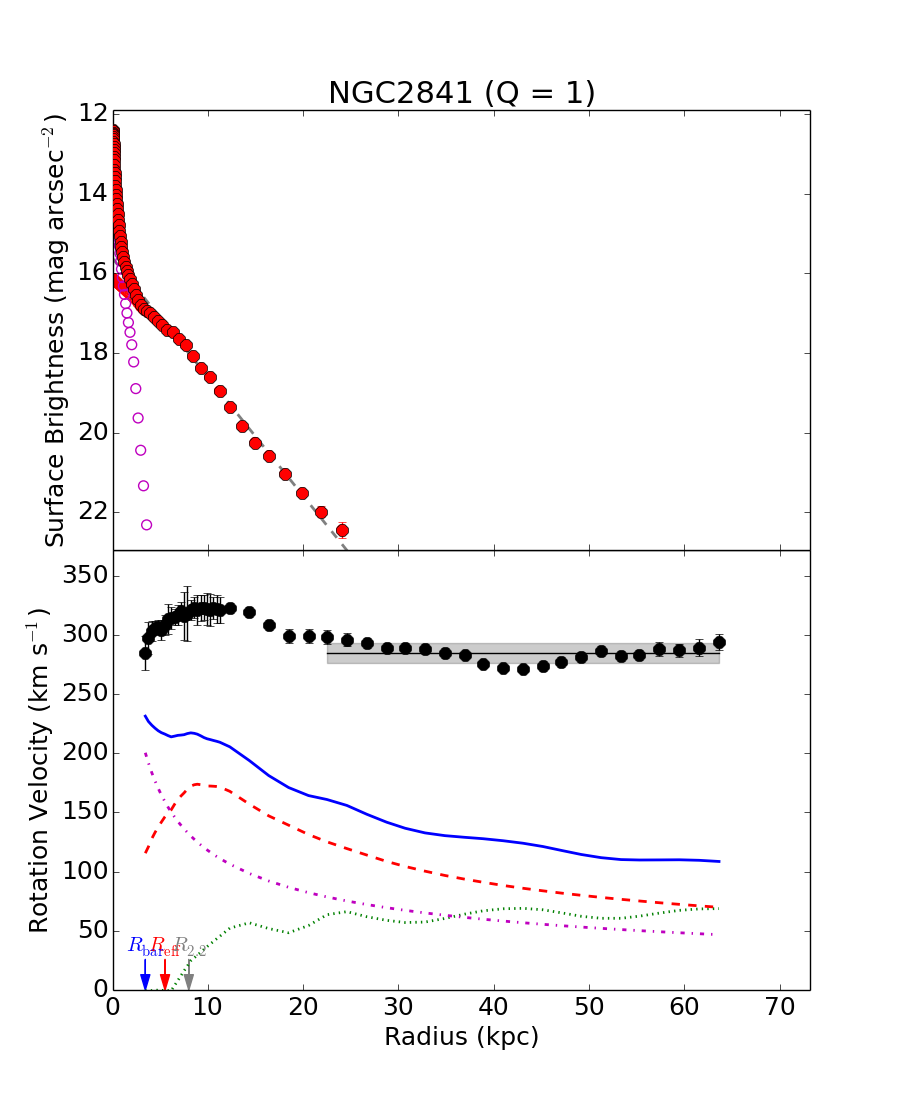
\includegraphics[scale=0.5]{pics/lamp1.png}
\end{figure}

\begin{figure}[H]
\centering 
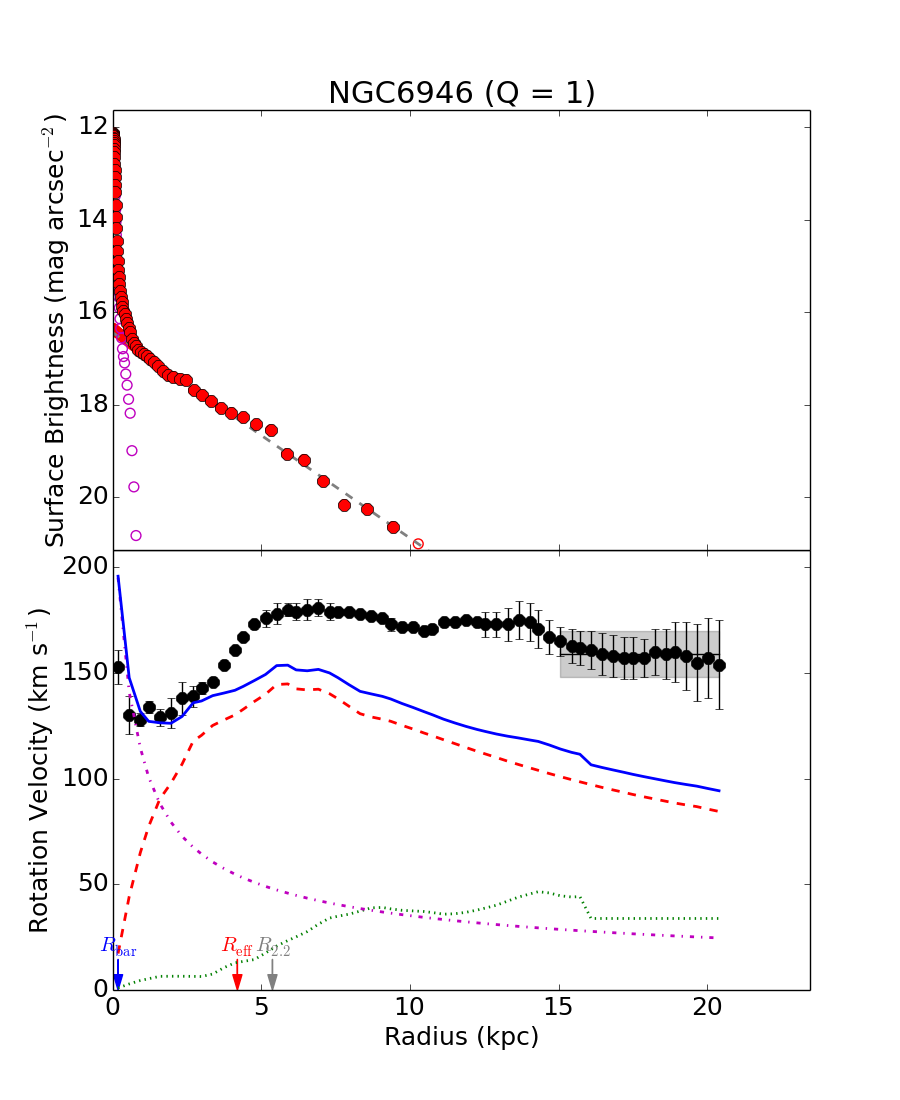
\includegraphics[scale=0.5]{pics/lamp2.png}
\end{figure}

\begin{figure}[H]
\centering 
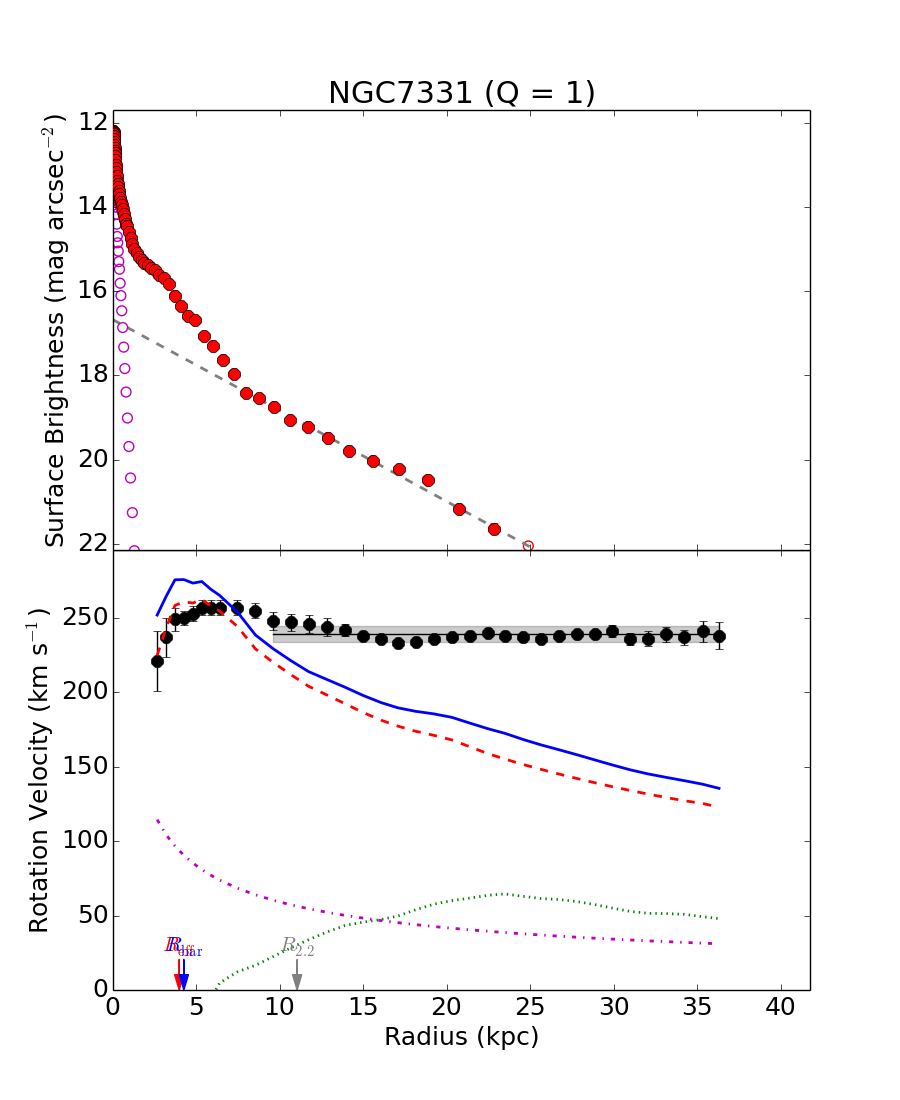
\includegraphics[scale=0.5]{pics/lamp3.png}
\end{figure}


\end{document}